\documentclass[usenames,dvipsnames,t]{beamer}

\usepackage[english]{babel}
\usepackage[utf8]{inputenc}
\usepackage{amsmath,amsthm, amssymb, latexsym}
\usepackage{amssymb}
\usepackage{color}
\usepackage{tikz}
\usepackage{standalone}
\usepackage{minted}
\usepackage{fontawesome}
\usepackage{setspace}
\usepackage{rotating}
\usepackage{booktabs}

\RecustomVerbatimEnvironment{Verbatim}{BVerbatim}{}
\definecolor{DarkGray}{RGB}{5, 66, 81}
\definecolor{DarkerGray}{RGB}{3, 22, 27}
\definecolor{Myorange}{RGB}{255, 165, 0}

\usemintedstyle{native}

\usetikzlibrary{shapes.arrows, positioning, arrows, decorations.pathreplacing,
angles, quotes, decorations.pathmorphing, fit, backgrounds,
calc, arrows.meta, automata, backgrounds}

\tikzstyle{background}=[solarizedRed, rectangle, draw, inner sep=0.7mm,
           rounded corners=1mm, ultra thick]
\tikzset{
    ultra thick/.style={line width=3pt},
    super thick/.style={line width=6pt}
}
\newcommand*\circled[1]{\tikz[baseline=(char.base)]{
            \node[shape=circle,draw,inner sep=2pt] (char) {#1};}}

\usetikzlibrary{matrix}

\usecolortheme[dark,accent=cyan]{solarized}
\beamertemplatenavigationsymbolsempty
\setbeamerfont{block title}{size=\Large}
\usepackage[orientation=landscape,size=a1,scale=1.4]{beamerposter}
\newcommand{\R}{\mathbb{R}}

\renewcommand{\arraystretch}{0.8}

\addtobeamertemplate{block begin}{%
  \setlength{\textwidth}{.5\textwidth}%
}{}

\addtobeamertemplate{block alerted begin}{%
  \setlength{\textwidth}{.5\textwidth}%
}{}

\addtobeamertemplate{block example begin}{%
  \setlength{\textwidth}{.5\textwidth}%
}{}
\setbeamerfont{block body}{size=\footnotesize}
\setbeamercolor{block title}{use=structure,fg=black,bg=purple!75!black}
\setbeamercolor{block body}{use=structure,fg=white,bg=white!20!white}
%%%%%%%%%%%%%%%%%%%%%%%%%%%%%%%%%%%%%%%%%%%%%%%%%%%%%%%%%%%%%%%%%%%%%%%%%%%%%%%
\begin{document}

%%%%%%%%%%%%%%%%%%%%%%%%%%%%%%%%TITLE%%%%%%%%%%%%%%%%%%%%%%%%%%%%%%%%%%%%%%%%%%%
\begin{columns}
    \begin{column}{.02\linewidth}
    \end{column}
    \begin{column}{.1\linewidth}
        \vspace{1cm}

        \begin{center}
        
\includegraphics[width=.7\textwidth]{static/mpi.jpg}
        \end{center}
    \end{column}
    \begin{column}{.7\linewidth}
    \vspace{1.5cm}

    \centering
    \vspace{1cm}
    \textbf{\textcolor{orange}{\Huge A bibliometric study of the Iterated Prisoner's Dilemma}}
    \vspace{1cm}

    \textbf{\textcolor{orange}{\large \circled{1} We collect scholarly data \circled{2} We classify abstracts into research topics \circled{3} We explore collaboration using co-authorship}}
    \end{column}
    \begin{column}{.1\linewidth}
        \vspace{1cm}

        \begin{center}
            
\includegraphics[width=.7\textwidth]{static/cardiff_uni_logo}
        \end{center}
        \end{column}
    % \begin{column}{.23\linewidth}

    %     \includestandalone[width=\textwidth]{static/memory_one}
    % \end{column}
    \begin{column}{.02\linewidth}
    \end{column}
\end{columns}
\vspace{1cm}

\hrule height 3pt
\vspace{1cm}

% %%%%%%%%%%%%%%%%%%%%%%%%%%%FIRST COLUMN%%%%%%%%%%%%%%%%%%%%%%%%%%%%%%%%%%%%%%%

% \begin{minipage}{.33\linewidth}
% \begin{center}
%     \Large\textcolor{orange}{How do we collect data on a field?}
% \end{center}
% \end{minipage}
% \begin{minipage}{.33\linewidth}
% \begin{center}
%     \Large\textcolor{orange}{What do people write about?}
% \end{center}
% \end{minipage}
% \begin{minipage}{.33\linewidth}
% \begin{center}
%     \Large\textcolor{orange}{Is the field of cooperation a collaborative field?}
% \end{center}
% \end{minipage}
\vspace{1cm}

\begin{columns}
\begin{column}{.33\linewidth}
    \begin{center}
    \textbf{\Large\textcolor{orange}{\textsc{\circled{1} HOW \& FROM WHERE}}}
    \vspace{.5cm}

    \textbf{\Large\textcolor{orange}{\textsc{DO WE COLLECT DATA?}}}
    \end{center}
    \vspace{1cm}

    \begin{center}
        \includestandalone[width=.45\textwidth]{static/arcas_diagram}
    \end{center}

    \begin{figure}
    \centering
    \begin{minipage}{4cm}
        \setbeamercolor{postit}{bg=solarizedBase00}
        \begin{beamercolorbox}[ht=.7cm, sep=.2em, wd=22cm, rounded=true]{postit}
        \textcolor{solarizedBase03}{\scriptsize
         \textbf{\textsc{RCAS is an open source tool with which we collect articles' meta-data in a few lines of code}}}
        \end{beamercolorbox}
    \end{minipage}
    \vspace{1cm}

    \begin{minted}
        [
        autogobble=true,
        framesep=2mm,
        fontsize=\footnotesize,
        ]
        {python}
    >>> import arcas
    
    >>> api = arcas.Arxiv()
    >>> params = api.parameters_fix(title="EHBEA",
                                    abstract="EHBEA",
                                    records=1)
    
    >>> url = api.create_url_search(params)
    >>> request = api.make_request(url)
    >>> root = api.get_root(request)
    >>> raw_article = api.parse(root)
    >>> article = api.to_dataframe(raw_article[0])
    \end{minted}
    \end{figure}
    \vspace{1cm}

    \begin{center}
        \scriptsize{\textcolor{orange}{keywords}: prisoner's dilemma, prisoners dilemma,
        prisoner dilemma, prisoners evolution, prisoner game theory}\\
        \vspace{.2cm}
        \scriptsize{\textcolor{orange}{search field}: title, abstract, text}\\
        
        \vspace{-.7cm}
        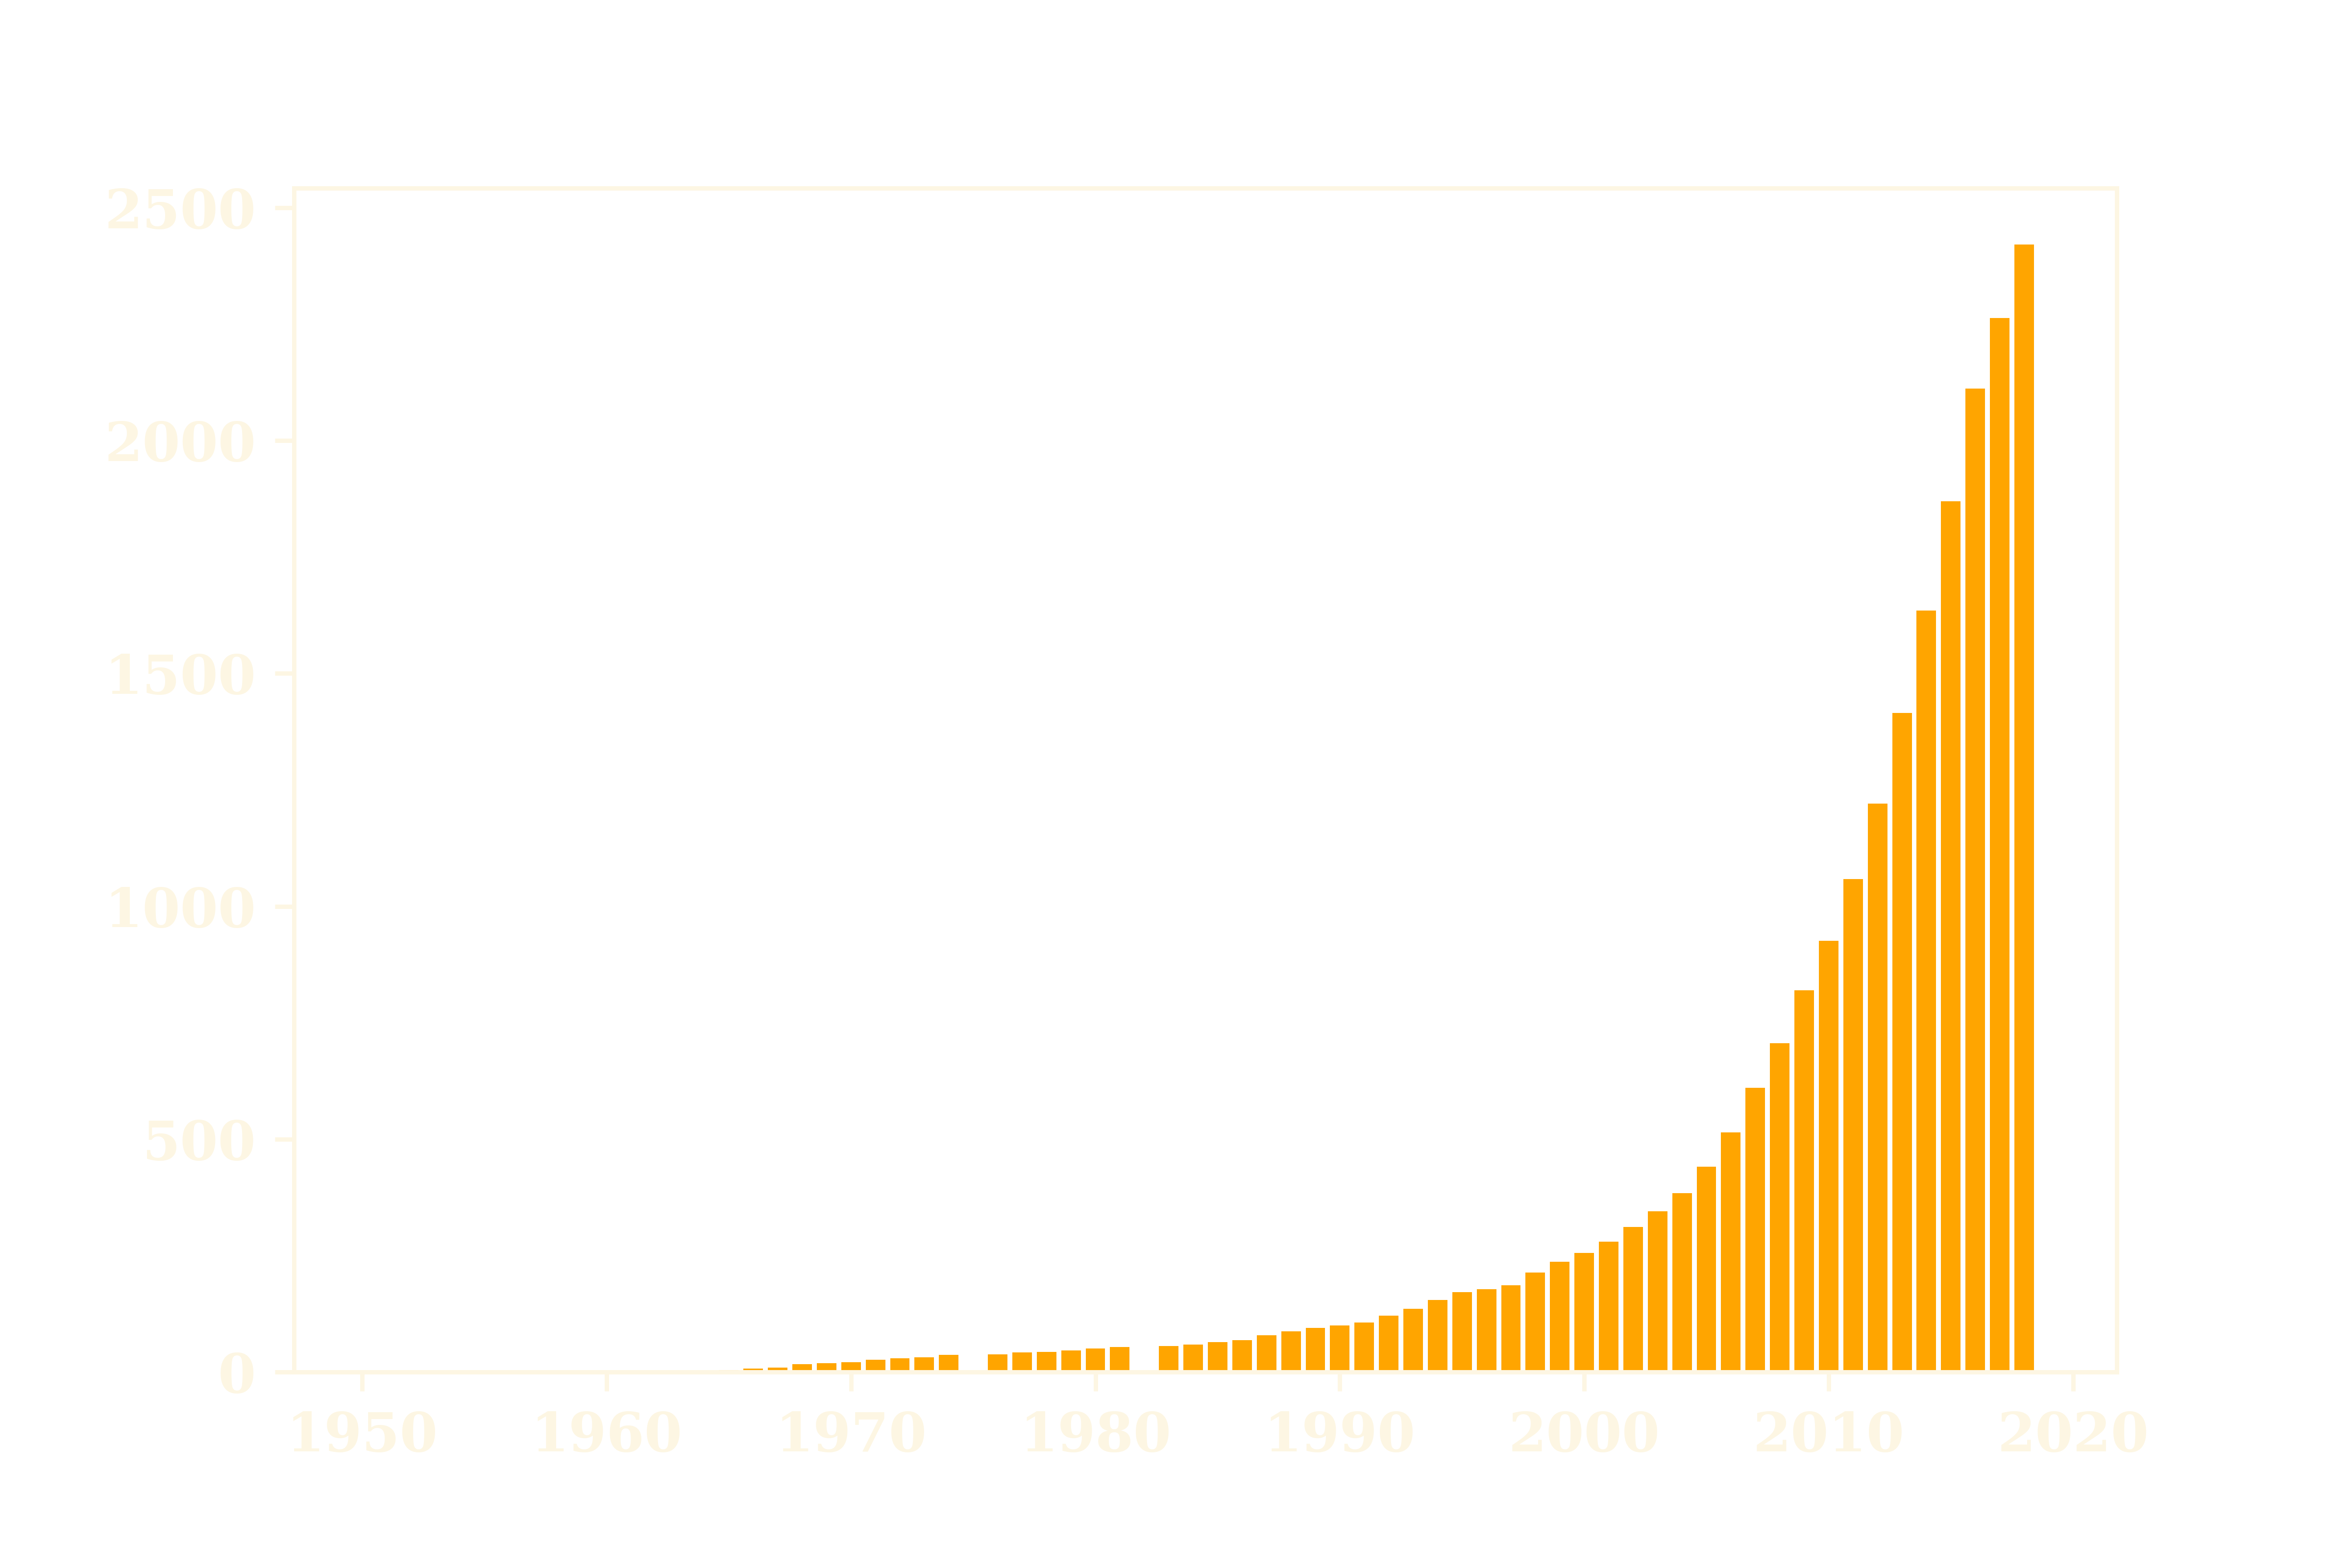
\includegraphics[width=.8\textwidth]{static/articles.png}
    \end{center}
\end{column}
% %%%%%%%%%%%%%%%%%%%%%%%%%%%SECOND COLUMN%%%%%%%%%%%%%%%%%%%%%%%%%%%%%%%%%%%%%%%
\vrule width 3pt
\begin{column}{.33\linewidth}
    \begin{center}
        \textbf{\Large\textcolor{orange}{\circled{2} \textsc{WHAT DO RESEARCHERS}}}
        \vspace{.5cm}
    
        \textbf{\Large\textcolor{orange}{\textsc{WRITE ABOUT?}}}
    \end{center}
    % \colorbox{solarizedBase2}{{\begin{minipage}[t][.7\textheight][t]
    %     {\dimexpr1\textwidth-3\fboxsep-2\fboxrule-5pt\relax}
    \vspace{1cm}
    \centering
    \begin{minipage}{4cm}
        \setbeamercolor{postit}{bg=solarizedBase00}
        \begin{beamercolorbox}[ht=.7cm, sep=.2em, wd=9.3cm, rounded=true]{postit}
        \textcolor{solarizedBase03}{\small
         \textbf{\textsc{Latent Dirichlet Allocation}}}
        \end{beamercolorbox}
    \end{minipage}
    \vspace{1cm}

    \begin{center}
        \includestandalone[width=.45\textwidth]{static/lda}
    \end{center}
    \vspace{1cm}

    \begin{center}
        \includestandalone[width=.8\textwidth]{static/topics}
    \end{center}

    \begin{center}
        \includestandalone[width=.8\textwidth]{static/topics}
    \end{center}

    \vspace{1cm}
% \end{minipage}}}
\end{column}
\vrule width 3pt
% %%%%%%%%%%%%%%%%%%%%%%%%%%%THIRD COLUMN%%%%%%%%%%%%%%%%%%%%%%%%%%%%%%%%%%%%%%%
\begin{column}{.33\linewidth}
    \begin{center}
        \textbf{\Large\textcolor{orange}{\textsc{IS THE FIELD OF COOPERATION}}}
        \vspace{.5cm}
    
        \textbf{\Large\textcolor{orange}{\textsc{A COOPERATIVE FIELD?}}}
    \end{center}
    \vspace{1.5cm}

    % \begin{center}
    %     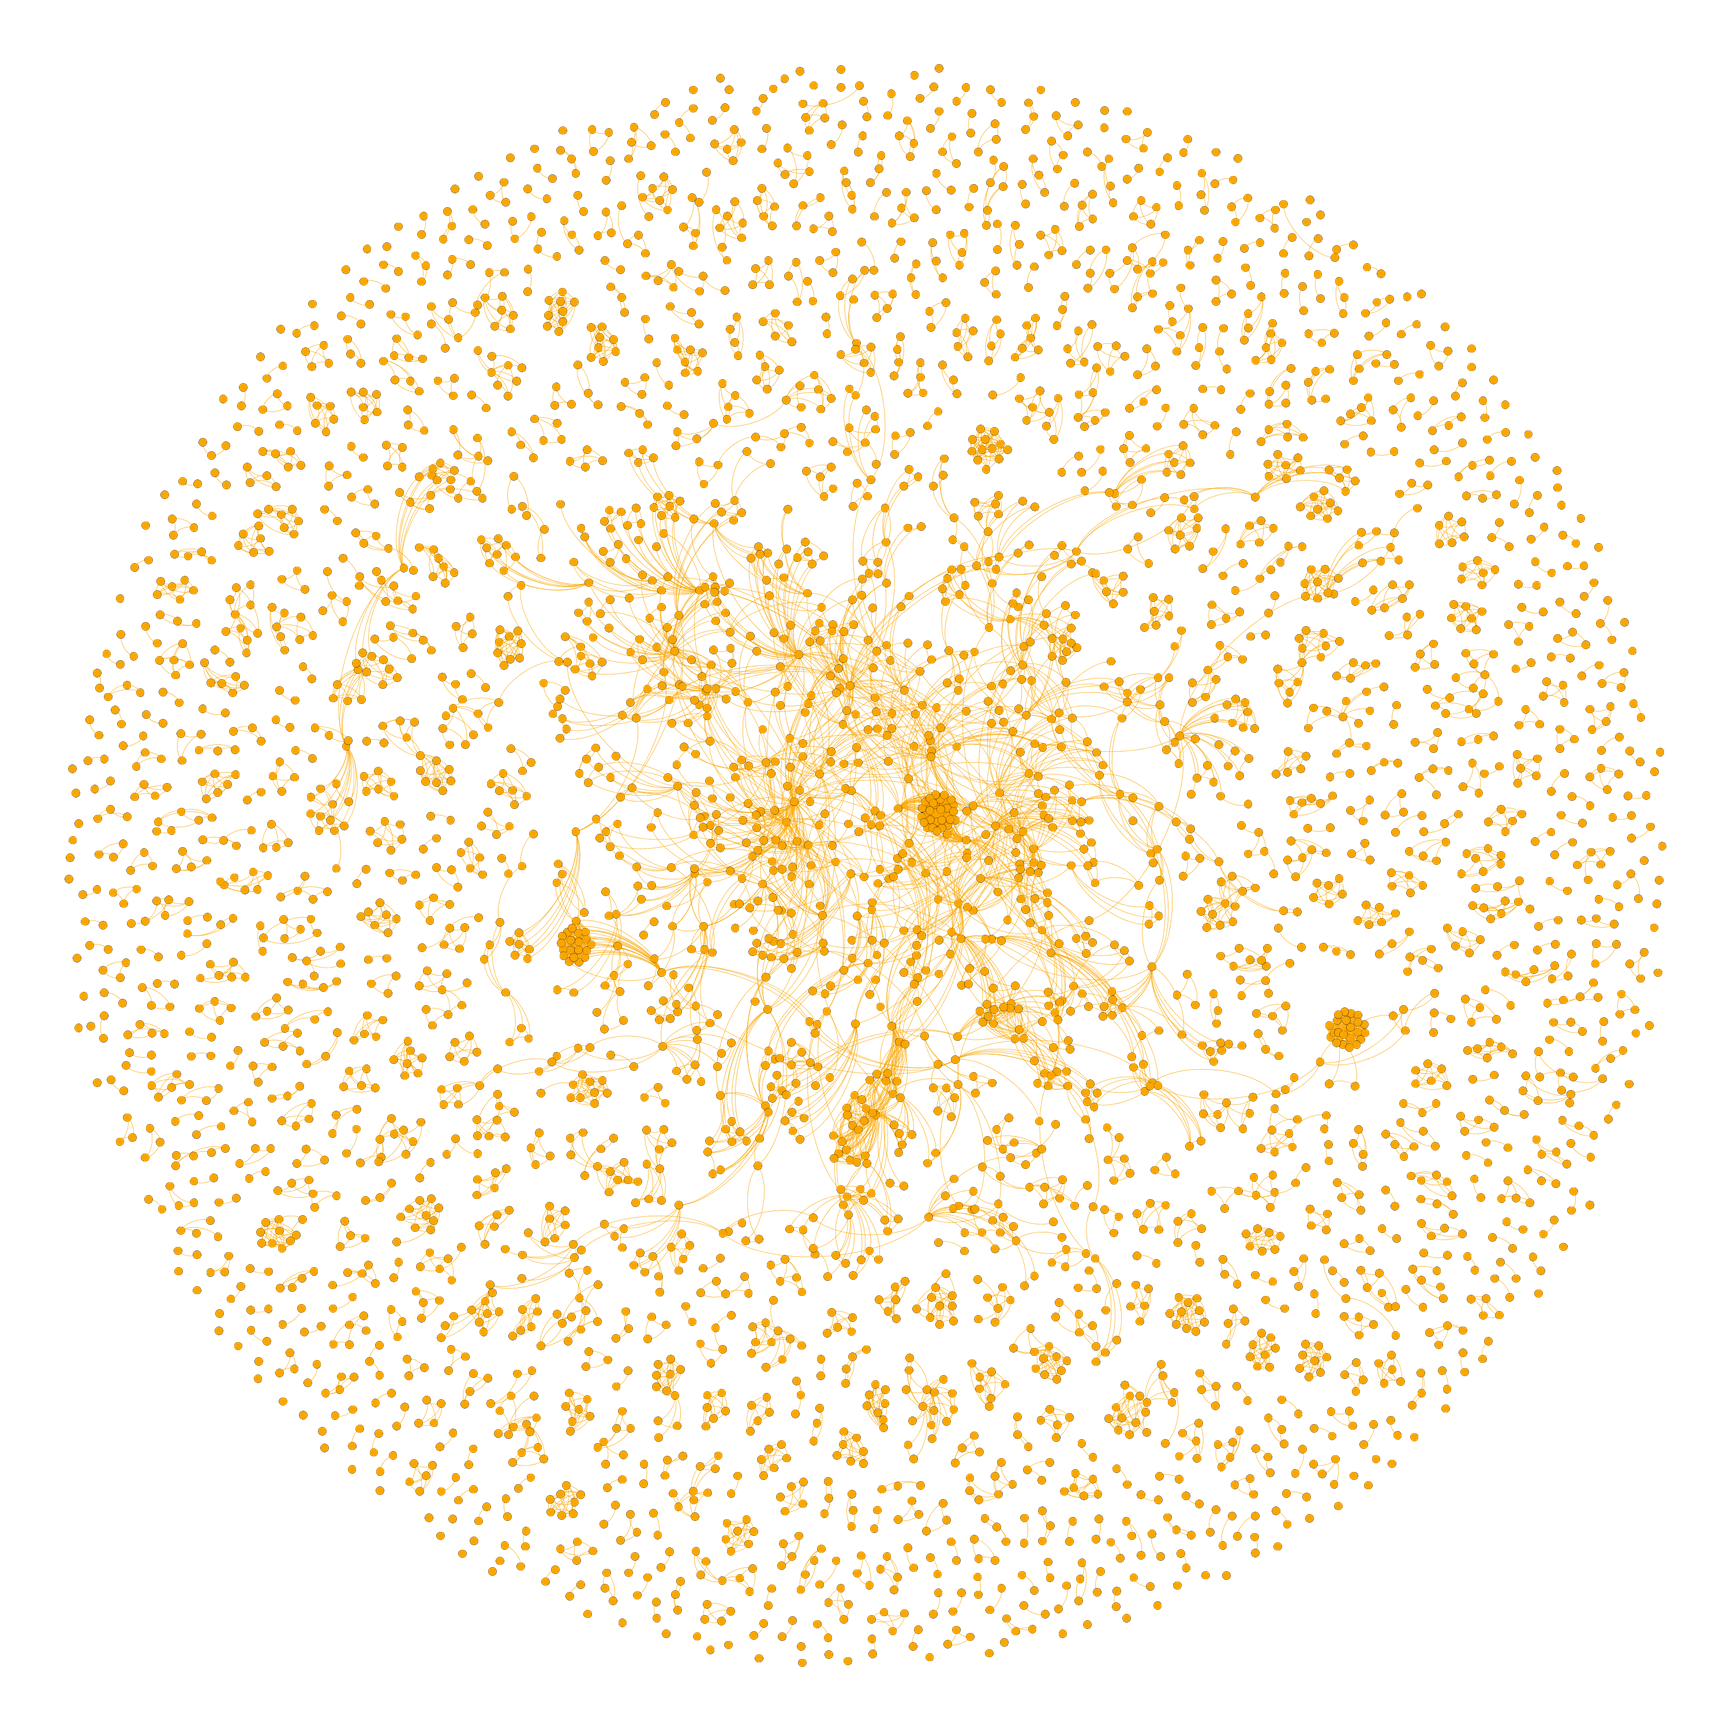
\includegraphics[width=.7\textwidth]{static/pd.png}
    % \end{center}

    \begin{center}
        \includegraphics[width=.6\textwidth]{static/degree_dist.png}
        \vspace{1cm}

        \small{
            $\bullet$ A
            \vspace{.2cm}

            $\bullet$ B
            \vspace{.2cm}
            
            $\bullet$ C}
    \end{center}

    % \Large{How does this compare?}
    % \resizebox{\textwidth}{!}{%
    % \begin{tabular}{lrrrrrrrrrr}
    %     \toprule
    %     {} &  \# Nodes  &   \% Isolated nodes &  \# Connected components &  Size of largest component &  Av. degree &  \# Communities &  Clustering coeff \\
    %     \midrule
    %     $G$              &     4221 &             8.0 &                    1157 &                        796 &       3.621 &           1177 & 0.666 \\
    %     Auction Games    &     5362 &             8.4 &                    1469 &                       1348 &       2.932 &           1493 & 0.599 \\
    %     Price of Anarchy &     1315 &            12.5 &                     406 &                        221 &       2.969 &            414 & 0.626 \\
    %     \bottomrule
    %     \end{tabular}}
    \vspace{1cm}
\end{column}
\end{columns}

\vspace{.5cm}

\hrule height 3pt
%%%%%%%%%%%%%%%%%%%%%%%%%%%%%%%%%%%%%INFO%%%%%%%%%%%%%%%%%%%%%%%%%%%%%%%%%%%%%%%
\begin{columns}
    \begin{column}{.2\linewidth}
        \vspace{0.3cm}

        \centering
        \textbf{ \faTwitter \ NikoletaGlyn \& \faTwitter \ VinceKnight}
    \end{column}
    \begin{column}{.6\linewidth}
        \vspace{0.3cm}

        \centering
        \textbf{ This work was supported by the European Research Council Starting Grant 850529 (E-DIRECT)}
    \end{column}
    \begin{column}{.2\linewidth}
        \vspace{0.3cm}

        \centering
        \textbf{ \faGithub \ Nikoleta-v3}
    \end{column}
\end{columns}
\end{document}
